
\section{Operads and props} \label{s:operads and props}

In this section we review the basic notions of operads and props.
For a more complete presentation we refer the reader to, for example, \cite{markl2008props}.

\subsection{Symmetric (bi)modules}

Let $\S$ be the category whose objects are the natural numbers and whose set of morphisms between $m$ and $n$ is empty if $m \neq n$ and is otherwise the symmetric group $\S_n$.
A \textit{left $\S$-module} (resp. \textit{right} $\S$-\textit{module} or $\S$-\textit{bimodule}) is a functor from $\S$-(resp. $\S^\op$ or $\S \times \S^\op$) to $\Ch$.
In this paper we prioritize left module structures over their right counterparts. As usual, taking inverses makes both perspectives equivalent.
We respectively denote by $\smod$ and $\sbimod$ the categories of left $\S$-modules and of $\S$-bimodules with morphisms given by natural transformations.

The group homomorphisms $\S_n \to \S_n \times \S_1$ induce a forgetful functor $\forget \colon \sbimod \to \smod$.
The similarly defined forgetful functor to right $\S$-modules will not be used.

\subsection{Composition structures}

We can define \textit{operads} and \textit{props} by enriching $\S$-modules and $\S$-bimodules with certain composition structures.
For a complete presentation of these concepts we refer to Definition~11 and 54 of \cite{markl2008props}.
Intuitively, using examples defined in the next subsection, operads and props can be understood by abstracting the composition structure naturally present in the left $\S$-module $\End^C$ (or right $\S$-module $\End_C$), naturally an operad, and the $\S$-bimodule $\End^C_C$, naturally a prop.
We remark that the prop structure on $\P$ restricts to an operad structure on $\forget(\P)$.

\subsection{Representations}

Given a chain complex $C$ define $\End^C$, $\End_C$ and $\End_C^C$ by
\begin{align*}
\End^C(r) &= \Hom(C, C^{\otimes r}),
& \End_C(r) &= \Hom(C^{\otimes r}, C),
& \End^C_C(r, s) &= \Hom(C^{\otimes r}, C^{\otimes s}),
\end{align*}
with their natural operad and prop structures respectively.
We remark that the forgetful functor $U$ sends $\End^C_C$ to $\End^C$.

Let $C$ be a chain complex, $\O$ an operad, and $\P$ a prop.
An $\O$-\textit{coalgebra} (resp. $\O$-\textit{algebra} or $\P$-\textit{bialgebra}) structure on $C$ is a structure preserving morphism $\O \to \End^C$ (resp. $\O \to \End_C$ or $\P \to \End_C^C$).

\subsection{$E_\infty$-operads and props}

An $\S$-module $M$ is said to be $E_\infty$-if for each $r$ the chain complex $M(r)$ is an algebraic model for the universal bundle $E\S_r$, i.e., it is free as an $\S_r$ module and its homology is that of a point.
An operad is said to be an $E_\infty$-operad if its underlying $\S$-modules is $E_\infty$, and following Boardman-Vogt \cite{boardman1973homotopy}, a prop $\P$ is said to be an $E_\infty$-prop if $U(\P)$ is an $E_\infty$-operad.

\subsection{Free constructions}

The free prop generated by an $\S$-bimodule can be constructed using isomorphism classes of directed graphs with no directed loops equipped with the following labeling structure.
We think of each directed edge as built from two compatibly directed half-edges. For each vertex $v$ of a directed graph $\Gamma$, we have the sets $in(v)$ and $out(v)$ of half-edges that are respectively incoming to and outgoing from $v$. Half-edges that do not belong to $in(v)$ or $out(v)$ for any $v$ are divided into the disjoint sets $in(\Gamma)$ and $out(\Gamma)$ of incoming and outgoing external half-edges.
For any positive integer $n$ let $\overline{n} = \{1,\dots,n\}$ and set $\overline{0} = \emptyset$.
The labeling is given by bijections
\[
\overline{m} \to in(\Gamma), \qquad
\overline{n} \to out(\Gamma),
\]
and, for every vertex $v$,
\[
\overline{p} \to in(v), \qquad
\overline{q} \to out(v).
\]
We refer to the isomorphism classes of such labeled directed graphs as $(n,m)$\textit{-graphs} and use graphs immersed in the plane to represent them, please see \cref{f:immersion}.
The set of $(m,n)$-graphs has an action of $\S_n \times \S_m^{\op}$ given by relabeling of incoming and outgoing external half-edges.
The collection $\{\G(m,n)\}_{m,n \geq 0}$ is equipped with a composition structure induced by grafting and disjoint union.
The free prop generated by an $\S$-bimodule is constructed using $M$ to decorate the vertices of $(m,n)$-graphs.
Please consult \cite{markl2008props} or \cite{fresse2010props} for a complete presentation.
The free operad generated by an $\S$-module is constructed similarly using only $(1,m)$-graphs.

The free prop functor can be composed with the free $\S$-bimodule functor,
\[
\big\{ S(m,n) \big\}_{m,n \geq 0} \, \mapsto \, \big\{ \S_n \times S(m,n) \times \S_m \big\}_{m,n \geq 0}
\]
and we assume this has been done whenever a free prop is described in terms of a bigraded set of generators.

\begin{figure}
	\boxed{\begin{tikzpicture}[scale=.6]
\draw (1,3.7) to (1,3); 

\draw (1,3) to [out=205, in=90] (0,0);

\draw [shorten >= 0cm] (.6,2.73) to [out=-100, in=90] (2,0);

\draw [shorten >= .15cm] (1,3) to [out=-25, in=30, distance=1.1cm] (1,1.5);
\draw [shorten <= .1cm] (1,1.5) to [out=210, in=20] (0,1);

\node at (1,3.9){};
\node at (0,-.32){};
\node at (2,-.32){};

\node at (3,1.5){$\sim$\ \ \ };
\end{tikzpicture}
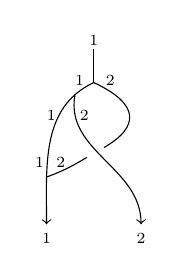
\begin{tikzpicture}[scale=.6]
\draw (1,3.7) to (1,3); 

\draw [->](1,3) to [out=205, in=90] (0,0);

\draw [shorten >= 0cm,->] (.6,2.73) to [out=-100, in=90] (2,0);

\draw [shorten >= .15cm] (1,3) to [out=-25, in=30, distance=1.1cm] (1,1.5);
\draw [shorten <= .1cm] (1,1.5) to [out=210, in=20] (0,1);


\def\x{.8}

\node[scale=\x] at (1,3.9){$\scriptstyle 1$};

\node[scale=\x] at (.7,3.05){$\scriptstyle 1$};
\node[scale=\x] at (1.35,3.05){$\scriptstyle 2$};

\node[scale=\x] at (.1,2.3){$\scriptstyle 1$};
\node[scale=\x] at (.8,2.3){$\scriptstyle 2$};

\node[scale=\x] at (-.15,1.3){$\scriptstyle 1$};
\node[scale=\x] at (.3,1.3){$\scriptstyle 2$};

\node[scale=\x] at (0,-.3){$\scriptstyle 1$};
\node[scale=\x] at (2,-.3){$\scriptstyle 2$};
\end{tikzpicture}}
	\caption{Immersed graphs represent labeled directed graphs with the direction implicitly given from top to bottom and the labeling from left to right.}
	\label{f:immersion}
\end{figure}

\subsection{The prop $\M$}

We now review the definition of the finitely presented $E_\infty$-prop $\M$ which, given its small number of generators and relations, is well suited to define $E_\infty$-structures.
This was already done for simplicial sets in \cite{medina2020prop1} where $\M$ was introduced.
In the next section we will do so for cubical sets.

\begin{definition} [Definition 3.1 in \cite{medina2020prop1}]
	Let $\M$ be the quotient of the free prop generated by
	\[
	\counit\,, \hspace*{.6cm} \coproduct\,, \hspace*{.6cm} \product,
	\]
	by the prop ideal generated by the relations
	\[
	\productcounit, \hspace*{.6cm} \leftcounitality\,, \hspace*{.6cm} \rightcounitality\,,
	\]
	where the first two generators are in degree $0$ and the third in degree $1$, with boundaries
	\[
	\partial\ \counit = 0,
	\hspace*{.6cm}
	\partial\ \coproduct = 0,
	\hspace*{.6cm}
	\partial\ \product = \ \boundary\,.
	\]
\end{definition}

\begin{proposition} [Theorem 3.3. in \cite{medina2020prop1}]
	The prop $\M$ is an $E_\infty$-prop.
\end{proposition}